\section{РЕШЕНИЕ}

Поиск оценки неизвестных параметров функции методом наименьших квадратов
вычисляется по формуле~\ref{eq:mnk}.
\begin{align}
\label{eq:mnk}
  &\widehat{\overline{\theta}} = \overline{\theta}^{(0)} + (Q^T Q)^{-1} Q^T (Z - \Psi( \overline{\theta}^{(0)})), \\
  &Q = \Psi'(\overline{\theta}^{(0)}) = \dfrac{d}{d\overline{\theta}^{(0)}} \Psi(\overline{\theta}^{(0)}). \nonumber
\end{align}

В нашем случае матрица $ Q^T $ будет выглядеть следующим образом.
\[
  \left[
    \begin{array}{ccccc}
      q_{11} & q_{12} & q_{13} & q_{14} & q_{15}  \\
      q_{21} & q_{22} & q_{13} & q_{14} & q_{15}
    \end{array}
  \right]^T.
\]

Элементы $ q_{ij} $ имеют следующий вид:
\begin{align*}
  &q_{1i} = \dfrac{d}{da^{(0)}} \Psi (a^{(0)}) = \dfrac{d}{da^{(0)}} ae^{-\alpha x_i} = e^{-\alpha^{(0)} x_i}, \\
  &q_{2i} = \dfrac{d}{d\alpha^{(0)}} \Psi (\alpha^{(0)}) = \dfrac{d}{d\alpha^{(0)}} ae^{-\alpha x_i} = -a x_i e^{-\alpha^{(0)} x_i}.
\end{align*}


С учётом того, что $ \Psi = f(x) = ae^{-\alpha x_i} $, имеем:
\begin{align*}
  &q_{1i} = \dfrac{d}{da^{(0)}} \Psi (a^{(0)}) = \dfrac{d}{da^{(0)}} ae^{-\alpha x_i} = e^{-\alpha^{(0)} x_i}, \\
  &q_{2i} = \dfrac{d}{d\alpha^{(0)}} \Psi (\alpha^{(0)}) = \dfrac{d}{d\alpha^{(0)}} ae^{-\alpha x_i} = -a x_i e^{-\alpha^{(0)} x_i}.
\end{align*}

Примем за первоначальные значения $ a^{(0)} $ и $ \alpha^{(0)} $ решение
системы двух уравнений вида:
\[
  \left\{
    \begin{array}{c}
      ae^{-\alpha x_1} = y_1, \\
      ae^{-\alpha x_2} = y_2.
    \end{array}
  \right.
\]

Построим функцию $ f(x) $ при начальных значениях $ a $ и $ \alpha $. Затем
применим метод наименьших квадратов для отыскания наиболее оптимальных параметров
функции $ f(x) $. Покажем вид этих функций на рисунке~\ref{pic:appr}.
\begin{figure}[h!]
  \centering
  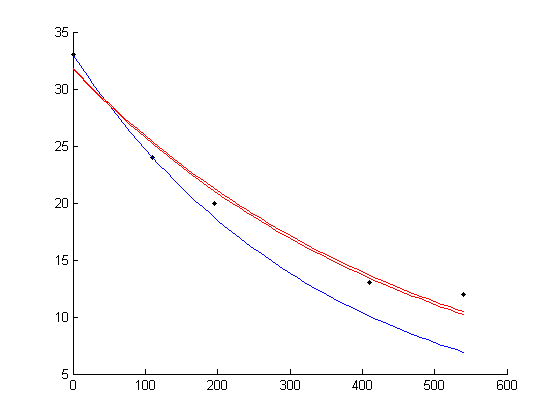
\includegraphics[width=1\linewidth]{pic/appr}
  \caption{Функция $ f(x) $ в зависимости от параметров}
  \label{pic:appr}
\end{figure}

\begin{table}[h!]
  \caption{Результаты вычислений}
  \label{tbl:results}
  \small{
    \centering
    \begin{tabular}{| p{0.1\textwidth} | p{0.4\textwidth} | p{0.4\textwidth} |}
      \hline

      & Первоначальные значения & Значения после 10 итераций МНК \\ \hline
      $a$       & $30{,}0000$ & $31{,}7516$ \\ \hline
      $\alpha$  & $0{,}0029$  & $0{,}0021$  \\

      \hline
    \end{tabular}
  }
\end{table}

Исходный код разработанной программы расположен в приложении~А.

\newpage

Зависимость оценки параметров $ a $ и $ \alpha $ от числа итераций приведена
на рисунках~\ref{pic:a_per_iter}~и~\ref{pic:alpha_per_iter}.
\begin{figure}[h!]
  \centering
  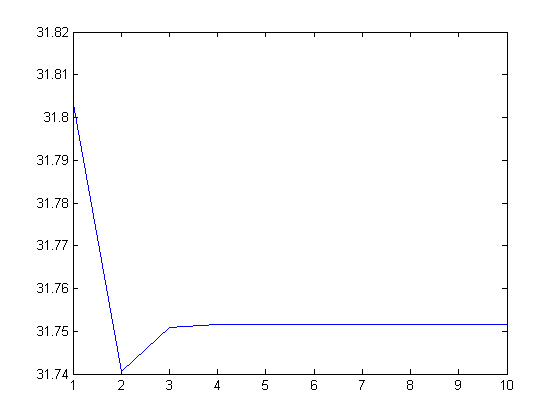
\includegraphics[width=0.77\linewidth]{pic/a_per_iter}
  \caption{Зависимость оценки параметра $ a $ от числа итераций}
  \label{pic:a_per_iter}
\end{figure}
\begin{figure}[h!]
  \centering
  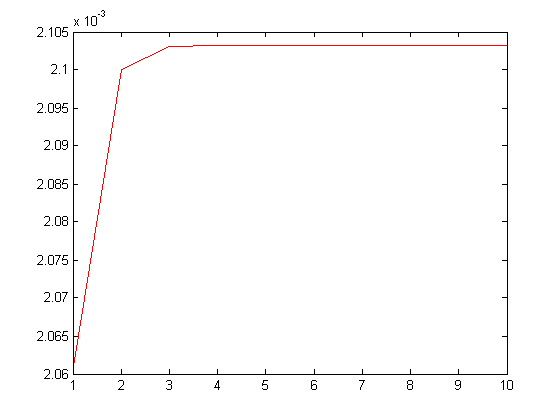
\includegraphics[width=0.77\linewidth]{pic/alpha_per_iter}
  \caption{Зависимость оценки параметра $ \alpha $ от числа итераций}
  \label{pic:alpha_per_iter}
\end{figure}
